\chapter{Maintaining and Compiling Bmad: Subversion and Gmake}
\label{c:svn_gmake}
\index{Subversion}
\index{Gmake}

This chapter describes how to access the code in the \bmad libraries 
and how to compile and link programs. There are two tools that are used
for this: \svn and \vn{gmake}. 

The \bmad distribution is stored in a \svn repository. \svn
is a widely used system for maintaining
documents. That is, by using \svn one can keep track of past
versions of documents, can keep a log of who, when, and why changes
occurred, can coordinate multiple people working on the same document,
etc.  Brief documentation about \svn can be obtained on Unix or Linux by
using the \vn{svn help} command. Complete documentation is available on
the web at
\begin{example}
  http://subversion.tigris.org
\end{example}
In the case of \bmad, most of the
documents are code files but, for example, the \bmad and \tao documentation is
also maintained under \svn.

\index{GNU}
\vn{Gmake} is the \vn{GNU} version of the \vn{make} system. Gmake is a
system whereby, after changes to program or library files are made,
only those files that need recompiling are recompiled. Considering the
time it can take to compile, this represents an enormous savings in
time. Actually, \vn{gmake} is more general than this amd the 
interested reader is referred to the
\vn{Gmake} documentation which can be obtained from the web at
\begin{example}
  http://www.gnu.org/software/make/manual/
\end{example}

\svn and \vn{gmake} are very sophisticated systems and the following
documentation only gives some of the basics to enable someone to
develop programs based upon \bmad.

%----------------------------------------------------------------------------
\section{Setting up SVN}
\label{s:svn_setup}
\index{SVN!setup}

\index{SVN!repository}
A ``repository'' is the place where \svn keeps the information
about the files (called ``sources'') it is maintaining. The repository
contains all the information to permit extracting previous versions of
the sources at any time. A \vn{project} is a collection of files. For example,
one project could be the book you are writing or a project could be the 
source code for a program.
A single repository can hold multipole \vn{projects} so
there is no reason to create multiple repositories. 

You don't need to setup a \svn repository for \bmad (it already
exists) but \svn can, in general, be useful for projects of all
stripes from writing a book to maintaining code. Therefore, this
section gives a brief overview of how to setup your own \svn
repository. Warning: Never modify a repository directly. Always use
the appropriate software tools.

The \svn repository is setup by creating a ``root'' directory
to hold everything using the command
\begin{example}
  svnadmin create <repository_root_dir> 
\end{example}
\vn{<repository_root_dir>} is the root directory name. \svn will create
\vn{<repository_root_dir>} and initialize it. For example:
\begin{example}
  svnadmin create /home/dcs/repos_root
\end{example}
will create the \vn{repos_root} directory and initialize it as a \svn repository.

The files for a \vn{project} can be devided up among multiple directories. 
The recommended directory tree structure for a project is to have three 
top-level directories named \vn{branches}, \vn{tags}, and \vn{trunk}. 
Initially, the \vn{trunk} directory should hold all of the project files
while the other two directories are empty (see the \svn documentation for
more information on why this is recommended).

When starting a project, the first step is to store in the repository
the initial version of the 
files that are to be maintained using the command
\begin{example}
  svn import <import_dir> <repository_project_dir> import -m "<comment>" 
\end{example}
\vn{<comment>} is the comment string associated with the initial source
files. Everything in the <import_dir> directory including all
subdirectories will be put into the \svn repository at
\vn{<repository_project_dir>}. \vn{<repository_project_dir>} must be a
sub-directory of \vn{<repository_root_dir>}.
\vn{<repository_project_dir>} must be an absolute path name. If the \svn
repository is local then \vn{<repository_project_dir>} must be have
\vn{file://} prepended to its name. For importing via the internet the
string \vn{https://} or \vn{http://} must be prepended. For example:
\begin{example}
  svn import ./this_dir file:///home/dcs/repos_root/my_novel -m "1st draft"
\end{example}
This example creates a subdirectory \vn{my_novel} within
the repository and imports into this directory the contents of \vn{./this_dir}.

Note: Since \svn will import all the files it finds, it is important
that ``extraneous'' files not be present. For example, compiled object
files should not be put in the repository and should therefore be
deleted before an import. If necessary, the files to be imported can be
copied to a temporary directory for the import.

%----------------------------------------------------------------------------
\section{Using SVN}
\label{s:svn_use}
\index{SVN}

Once a project has been set in the repository,
a local copy of the files in the
repository can be created using the ``checkout'' command
\begin{example}
  svn co <repository_project_dir> <local_project_dir>
\end{example}
This will make a directory \vn{<local_project_dir>} with everything in it.
Following the example of the previous section, the command
\begin{example}
  svn co file:///home/dcs/repos_root/my_novel my_novel
\end{example}
will create a \vn{my_novel} directory in your working directory.
In addition the local copy of the project  will contain directories
named \vn{.svn} which contains information necessary for maintanance.
The files in the \vn{.svn} directory should never be touched since
this could cause \svn to misbehave. 

You are free to modify the files you have checked out from the
repository. The files in the repository will not be affected by this.
At some point you may want to put your modified files into the
repository. The command to check--in the files is
\begin{example}
  svn ci -m <comment> <file_or_dir_name>
\end{example}
If \vn{<file_or_dir_name>} is a directory then \svn will check--in all
files of that directory and any sub--directories under it. If
\vn{<file_or_dir_name>} is not present then the current working
directory is used. \vn{<comment>} is a comment associated with the
modified files. If you omit the \vn{-m <comment>} option then \svn
will pop up an emacs window for you to type a comment in.
For example, if \vn{my_novel/file1} has been modified
and if \vn{my_novel} is the current directory, the command
\begin{example}
  svn ci -m "My First Revision"
\end{example}
will check-in \vn{file1} to the repository. The information printed to
the terminal when this command is executed looks like:
\begin{example}
  Sending    file1
  Transmitting file data ...
  Committed revision 2.
\end{example}
The latest state of this project in the repository is labeled 
revision \vn{2}.

If you want to know what files have been modified from what is in the
repository you use the command
\begin{example}
  svn stat -u
\end{example}
For an explanation of the output of this command use the command:
\begin{example}
  svn help stat
\end{example}

To see how a local file has been modified from what was checked out use
the command
\begin{example}
  svn diff <file_name>
\end{example}
The output of this command is independent of any modifications checked in
to the repository by other people.
To see how a local file has been modified from what is in the repository use the
command
\begin{example}
  svn diff -r HEAD <file_name>
\end{example}
The output of this command is in \vn{unified diff format} which is what you
would see using the Unix \vn{diff -u} command.

The command to delete a file is
\begin{example}
  svn delete <file>
\end{example}
The file will not actually be deleted from the repository until you do a
\vn{svn ci}.

%----------------------------------------------------------------------------
\Section{Using SVN with Bmad}

The \svn repository for \bmad contains \bmad and the associated
libraries (\sref{s:libs}). Periodically all the libraries are checked
out and compiled. This is called a \vn{release}. Typically the release
root directory is named after the creation date. For example, one release is:
\begin{example}
  /home/cesrulib/cesr_libs/OSF1_alpha/cesr_2005_0320_d
\end{example}
This is a release for the OSF True64 computers built on March 20,
2005. There needs to be different releases for different platforms,
and even with different compilers on the same platform, since the
compiled binary files will be different. Thus, at this time, there are
different releases on Linux for the two compilers in use
(Lahey--Fujitsu and Intel). It is important that if you are developing on
different platforms, or even developing with different compilers, that
you keep your binaries separate as well.

The latest release always has a soft link named \vn{devel}. There is
also a \vn{current} soft link that points to the last "stable" release
that is felt to be (relatively) bug free. The advantage to using the
\vn{devel} version over \vn{current} is that you get the latest bug
fixes (if any). The disadvantage is that it might not be as
stable. Typically people use the \vn{devel} release.

To initialize for \bmad, the \vn{CESRLIB} environmental variable needs
to be set to the desired release root directory and the appropriate
command file must be run. This command file is different for the
\vn{bash} and \vn{tcsh} shells. For example, with \vn{tcsh}, to run
the devel release put the following lines in your \vn{.login} file:
\begin{example}
  setenv CESRLIB devel
  source /home/cesrulib/bin/cesrdef
\end{example}
For \vn{bash} use
\begin{example}
    CESRLIB=devel
    . /home/cesrulib/bin/cesrdefs
\end{example}
Other releases can be used by setting \vn{CESRLIB} appropriately. To
see the names of all the releases look at the directory appropriate
for the compiler and platform which at present are
\begin{example}
  /home/cesrulib/cesr_libs/Linux_alpha       # Linux    Lahey
  /home/cesrulib/cesr_libs/Linux_i686        # Linux    Intel
  /home/cesrulib/cesr_libs/OSF1_alpha        # OSF      Intel
  /home/cesrulib/cesr_libs/CYGWIN_NT_i686    # Windows  Intel
  /home/cesrulib/cesr_libs/VMS_alpha         # VMS      HP
\end{example}

To see the logicals that are setup by the \vn{cesrdef(s)} command file
use the following command:
\begin{example}
  printenv | grep CESR
\end{example}
This will produce something like
\begin{example}
  CESRLIB=devel
  CESR_PLATFORM=OSF1_alpha
  CESR_BASE=/home/cesrulib/cesr_libs/OSF1_alpha
  CESR_CURRENT=/home/cesrulib/cesr_libs/OSF1_alpha/current
  CESR_DEVEL=/home/cesrulib/cesr_libs/OSF1_alpha/devel
  CESR_DOC=/home/cesrulib/cesr_libs/doc
  CESR_SVNROOT=/home/cesrulib/cesr_libs/svnroot
  CESR_REL=/home/cesrulib/cesr_libs/OSF1_alpha/devel
  CESR_CONFIG=/home/cesrulib/cesr_libs/OSF1_alpha/devel/config
  CESR_SVNSRC=/home/cesrulib/cesr_libs/OSF1_alpha/devel/svnsrc
  CESR_EXE=/home/cesrulib/cesr_libs/OSF1_alpha/devel/bin
  CESR_GMAKE=/home/cesrulib/cesr_libs/OSF1_alpha/devel/Gmake
  CESR_LIB=/home/cesrulib/cesr_libs/OSF1_alpha/devel/lib
  CESR_MOD=/home/cesrulib/cesr_libs/OSF1_alpha/devel/modules
  CESR_RUN=/home/cesrulib/cesr_libs/OSF1_alpha/devel/run
  CESR_UTIL=/home/cesrulib/cesr_libs/OSF1_alpha/devel/util
  CESR_INC=/home/cesrulib/cesr_libs/OSF1_alpha/devel/svnsrc/include
  CESR_PKG=/home/cesrulib/cesr_libs/OSF1_alpha/devel/packages
  CESR_CONST=/home/cesrulib/constants
\end{example}

The source code for the local libraries (\vn{Bmad}, \vn{cesr_utils},
\vn{recipes_f-90_LEPP}, and \vn{dcslib}) is in \vn{CESR_SVNSRC}. The
source code for the outside libraries (\vn{forest}, \vn{recipes},
\vn{PGPLOT}, and \vn{xsif}) is in \vn{CESR_PKG}. The
\vn{recipes_f-90_LEPP} library is the specially modified version of
Numerical Recipes (\sref{s:libs}) that can handle either single or
double precision reals. This is not to be confused with the original
single precision version (which is never compiled) \vn{recipes_f-90}
which is in \vn{CESR_PKG}. 

A web based viewer has been setup for \bmad. It can be accessed at
\begin{example}
  http://www.lns.cornell.edu/~cesrulib
\end{example}

Some programs are also maintained in the the \svn repository. some of
these are compiled and linked with a release. The executables are in
\vn{CESR_BIN}. The most notable is \vn{bmadz} which is the CESR
storage ring lattice design program.

If you just link against a release you don't need to check--out and
compile any of the \bmad source code. If you do need to do this the
next section will explain how this is done.

For people outside Wilson Laboratory who need a local copy of \bmad
there are what are called \vn{distributions}. A \vn{distribution} is
made by checking out the \bmad distribution and taring it into one
file for portability. \vn{Distributions} may be obtained from the
\bmad web page (\sref{s:libs}).

%----------------------------------------------------------------------------
\section{Compiling and Linking Bmad Programs}
\label{s:compile}

\begin{figure}[tb]
  \begin{centering}
  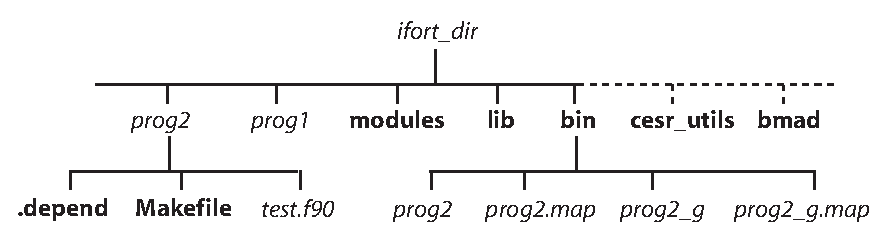
\includegraphics{devel-dir.eps}
  \caption[Standard Directory Structure for Bmad Programs.]
{Example of a directory structure for developing Bmad programs. Standardized
names are shown in bold. Italicized names are arbitrary.}
  \label{f:devel_dir}
  \end{centering}
\end{figure}

To facilitate the automatic compiling and linking of programs there is
a standard directory structure, an example of which is shown in
Figure~\ref{f:devel_dir}. In Figure~\ref{f:devel_dir} names in italics
have been arbitrarily chossen for the purposes of this example. Names
in bold are standardized names that will be the same between different
implementations of this directory structure.

\vn{ifort_dir} is the root development directory.  In
Figure~\ref{f:devel_dir} \vn{prog1} and \vn{prog2}
are directories for developing programs. Although only two program
directories are shown, there is no limit as to their number. Code
files can be put in a program directory or in sub--directories. The
\vn{lib} directory of for compiled libraries, the \vn{modules}
directory is for compiled Fortran modules, and the \vn{bin} directory
is for executable files. There can also be local copies of the
\vn{bmad} library and it subsidiary libraries (\sref{s:libs}).

\index{Gmake}
A program directory will always have a \vn{Makefile} file that is used
by \vn{gmake} to compile and link programs. Any local libraries will
also have their own \vn{Makefile} files. Program makefiles are
different from library makefiles and even two program makefiles can 
be different (see below).

Any given program directory can have one or multiple programs within
it. If it has only one program then to compile and link the program
use the command
\begin{example}
  gmake
\end{example}
the default \vn{gmake} behavior in this case is to name the executable
file after the program directory name and not the program file
name. For example, in Figure~\ref{f:devel_dir}, the executable made
from \vn{test.f90} in \vn{prog2} is
\vn{bin/prog2}. There are actually two different executables:
A \vn{production} executable and a \vn{debug} one. The \vn{debug}
executable has a \vn{_g} appended to the name so in this example its
name is \vn{bin/prog2_g}.  The production executable will run
much faster than the debug version (roughly a factor of 3 or so). The
debug version, however, can be used with a debug program to examine
the program as it is running.  The debug version of the program, just
like the production version, can be run without a debugger and this is
sometimes useful since the debug version will catch errors such as an
array index out of bounds that the production version would not.

Along with the executables, \vn{gmake} will make a \vn{.map} file for
each executable which shows where each routine that is part of the
program came from. The \vn{.map} files are are sometimes helpful in
debugging a program. For example, \vn{bin/prog2_g.map} is the
map file associated with \vn{bin/prog2_g}.

To save time, if only the \vn{production} executable is needed, the command
\begin{example}
  gmake production
\end{example}
can be used. To create only the debug version use
\begin{example}
  gmake debug
\end{example}
If there is more than one program in a program directory then the
\vn{gmake} syntax is
\begin{example}
  gmake MAIN_FILE=<program_file_name>
\end{example}
In this case the executable file will be named after the program file
name.

\index{.depend}
\vn{gmake} tries to cut compile and link time by only compiling and/or
linking when file are "out-of-date". Thus \vn{gmake} will only relink
the executable if the creation date of the executable is prior to the
creation dates of the object files that are linked. The dependency
rules that \vn{gmake} uses to decide if one file is dependent upon
another file are kept in a series of files in the \vn{.depend}
directory in a program directory. These dependency files are updated
whenever program files are changed but sometimes \vn{gmake} can become
confused (say if a local library is deleted that the local program
files depend upon) and if this happens the best way to reset things is
via the command
\begin{example}
  gmake clean
\end{example}
This removes the executables, object files and \vn{.depend} directory.

Generally one does not have to worry too much about how \vn{Gmake}
uses a \vn{Makefile} to compile programs but some knowledge is
essential. The operation of the \vn{Makefile} is to set some flags and
then, at the end of the \vn{Makefile}, a second makefile called
\vn{M.tail} is included. It is actually \vn{M.tail} that does all the
work. The \vn{Makefile} is divided up into documented sections.
One such section is:
\begin{example}
  #--------------------------------------------------------------
  # Provide the list of libraries required for linking this job.
  # All lists should be space delimited.
  #
  # LOCAL_LIBS    Local user-supplied libraries
  # CESR_LIBS     CESR libraries
  # PKG_LIBS      CESR outside packages libraries
  # CERN_LIBS     CERN libraries
  #
  # NOTE:  Search order is 
  #        1) locallib area  (typically ../lib)
  #        2) EXTRA_LIB area (optionally specified by the user)
  #        3) CESR_LIB area  (library area for currently specified 
  #                           CESR release)
  #        4) PKG_LIB area   (library area for outside CESR 
  #                           packages)
  #        5) CERN_LIB area  (CERN libraries)
  #--------------------------------------------------------------
  LOCAL_LIBS := 
  CESR_LIBS  := bmad dcslib cesr_utils recipes_f-90_LEPP
  PKG_LIBS   := forest pgplot
  CERN_LIBS  :=
  SYS_LIBS   :=
\end{example}
This section sets the libraries to be linked to the program. Often
link failures can be traced to missing libraries or libraries out of
order. For example, since the \vn{Bmad} library depends upon
\vn{dcslib}, \vn{bmad} must come first in the \vn{CESR_LIBS} list.

Another section in the \vn{Makefile} sets where the executable resides
\begin{example}
  #-------------------------------------------------------------
  # Generate the executable name - the default is \$(JOB) unless  
  # MAIN_FILE has been explicitly specified
  #-------------------------------------------------------------
  ifeq "$(strip $(MAIN_FILE))" ""
          EXE := ../bin/\$(JOB)
  else
    EXE := ../bin/\$(basename \$(notdir \$(MAIN_FILE)))
  endif
\end{example}
\vn{\$(JOB)} is the program directory. 

The standard debug program is called \vn{totalview}. \vn{totalview} is
put out by a company called Etnus and documentation on totalview can
be obtained from the web at
\begin{example}
  http://www.etnus.com
\end{example}

Local copies of \bmad and/or its subsidiary libraries are only
generally only needed in special circumstances. Problems can arise
with local libraries if they are not keep up-to-date with the
repository versions. For this reason it is best to remove local
libraries if they are no longer needed. The command for this is
\begin{example}
  gmake clean
\end{example}
Just removing the library code directory is not enough since modules
in the \vn{modules} directory and the library itself in the \vn{lib}
directory will remain. When compiling libraries it must be remembered
that there is a definite order to the compilation. This is due to the
fact that since Fortran modules are compiled, if a library has a
module that is used by a file in another library, the first library
must be compiled first. The order of libraries is
\begin{example}
  tao
  bmad
  dcslib
  recipes_f-90_LEPP
  cesr_utils, forest, XSIF 
\end{example}
The bottom most libraries must be compiled first.
